\section{Related Work}
\label{related}
Wir sind nicht die Ersten, die mit einer Kombination aus realer und virtueller Welt experimentieren. Es gibt schon einige etablierte Spiele, die beides erfolgreich verbinden. Auch in anderen Bereichen, wie der Medizin  oder der Industrie, wird �ber die erweiterte Realit�t geforscht \cite{azuma}. 
% ?? H�ufig wird es im Sinne von viralem Marketing zur Bewerbung eines neuen Produktes oder einer neuen Dienstleistung verwendet, ohne dieses direkt anzupreisen und ohne das Spiel als Werbeveranstaltung erkennen zu lassen.
Im folgenden Abschnitt werden Spiele, die Teilaspekte der entwickelten Spielideen umsetzen, kurz erl�utert.

\subsubsection{Ingress}
%Google selbst l�sst sich nicht lumpen und hat ein erfolgreiches Spiel implementiert. 
Ingress \cite{ingress} ist ein kooperatives interaktives Gesellschaftsspiel, welches sich auf der ganzen Welt abspielt. Zu Anfang w�hlt ein Spieler eines von zwei Teams. Von nun an geht es darum, mit seinem Team, �ber m�glichst gro�e �ffentliche Bereiche, virtuell zu gebieten. Au�erdem will die sogenannte "`Exotic Matter"' eingesammelt werden. Dies geschieht beides mit dem Scanner, wie das Spiel seine App nennt. Wenn man mit dem Scanner in die N�he von "`Exotic Matter"' kommt, wird dies eingesammelt und es k�nnen Aktionen bei in der N�he befindlichen "`Portalen"' durchgef�hrt werden. Ein Gebiet wird eingenommen, wenn mindestens drei Portale miteinander verlinkt sind.

\begin{figure}[htbp]
  \centering
    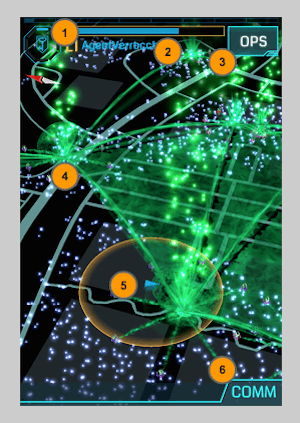
\includegraphics[width=0.5\textwidth]{2-Spielideen/2-3-Related_Work/ingress.png}
     \caption{der Scanner des Spiels Ingress. Auf der Karte werden "`Portale"' und das "`XM"' angezeigt und mit ihm k�nnen die Spieler untereinander agieren.
	(Quelle: \url{https://lh3.ggpht.com/OC9nlsdM9HjIUMJ4BHpUtLArV5qXyyqphqMHUjsmXp82rYcmSJgcp4v5DmXI5R7eB2z1fckH=w300})
		}
\end{figure}


\subsubsection{Pacman auf Google-maps}

%Ein weiteres kleines Minispiel, welches sich Google hat einfallen lassen, lie� sich nur eine bestimme Zeit lang spielen. 

Um den 1. April 2015 konnte man auf der normalen Google-Maps Seite die Stra�enkarte in ein Pacman-Spiel \cite{pacman} verwandeln und sich somit durch seine eigene (virtuelle) Stadt mit dem kleinen gelben Kreis fressen. 
Dies ist zwar nur ein Videospiel, dass vollst�ndig virtuell (ohne aktive Bewegungen in der Realit�t) gespielt wird, jedoch wird hier eine reale Karte als Spielfeld verwendet, was in unseren Implementationen ebenfalls ein wichtiger Punkt ist.
 
%Dies ein eher simples Beispiel f�r die Einf�hrung der realen Welt in ein virtuelles Spiel, da hier lediglich die Stra�enkarten in das Spiel integriert wurden. �hnlich den erarbeiteten Spielideen werden bei dieser Anwendung virtuelle Objekte auf einer Karte angezeigt.

\begin{figure}[htbp]
  \centering
    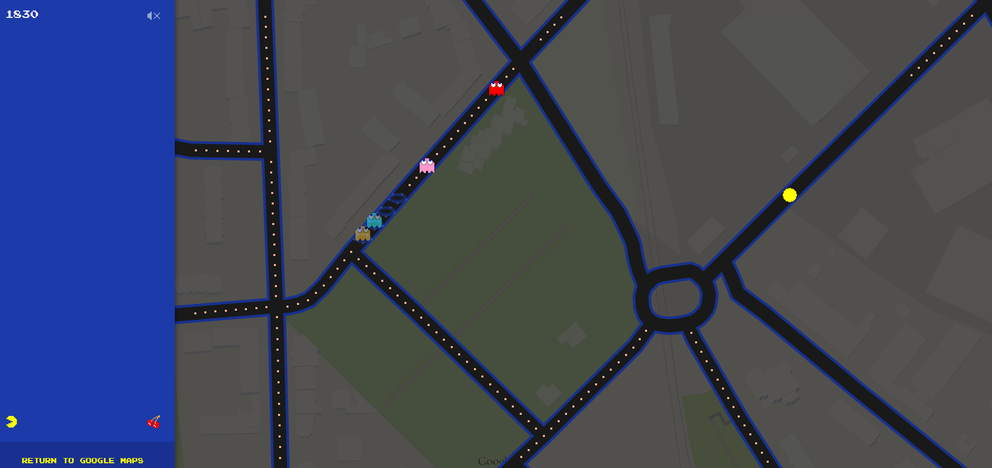
\includegraphics[width=0.9\textwidth]{2-Spielideen/2-3-Related_Work/pacman.png}
     \caption{Pacman auf Googlemaps
	(Quelle: \url{http://media2.giga.de/2015/03/pacman-google-maps-rcm992x0.png})
		}
\end{figure}


\subsubsection{Twinkomplex}

Eine andere Idee hatte der Entwickler von TwinKomplex \footnote{\url{http://twinkomplex.browsergames.de/}}. Er l�sst den Spieler in die Rolle eines Agenten schl�pfen. Dieser wird, mit Hilfe von Google-Maps und Open-Source-Daten, virtuell durch echte Schaupl�tze gef�hrt um F�lle zu l�sen. Hier wird die reale Welt in ein virtuelles Spiel eingearbeitet.

\begin{figure}[htbp]
  \centering
    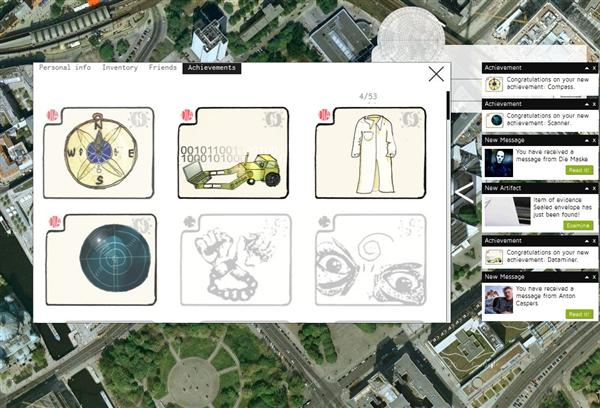
\includegraphics[width=0.65\textwidth]{2-Spielideen/2-3-Related_Work/twinkomplex.png}
     \caption{Screenshot des Spiels TwinKomplex. Auf einer reellen Karte gilt es Dinge zu finden bzw. mit Hilfe von einigen Utensilien einen Fall zu l�sen.
		(Quelle: \url{http://www.onlinegameslist.org/wp-content/uploads/2012/01/twinkomplex-game-achievements.jpg})
		}
\end{figure}

\subsubsection{Geocaching}

%Geocaching wird durch eine stark wachsende Gemeinschaft vertreten. Es gibt bereits �ber 2.630.700 "`Caches"' auf der Welt \footnote{\url{https://www.geocaching.com/play}}.  
Geocaching ist eine Art Schnitzeljagd. Mithilfe von GPS-Daten und Ger�ten, die einem dabei behilflich sein k�nnen (z.B. Smartphone), gilt es von anderen Mitspielern Verstecke (Caches) zu finden. Meist sind in diesen Caches Logb�cher und/oder Tauschgegenst�nde versteckt. Auch R�tsel, die zu einem n�chstes Cache f�hren sind �blich. Oft sind zusammenh�ngende Folgen von Verstecken thematisch gestaltet.
Geocaching hat eine gro�e Community und ist viel mehr auf Engagement der Community-Mitglieder direkte und indirekte soziale Interaktion ausgelegt, als die anderen vorgestellten Beispiele \cite{ohara}.
�hnlich den erarbeiteten Spielideen werden beim Geocaching GPS-Daten zur Orientierung verwendet.
%Wichtig beim Spielen von Geocaching ist, dass die Menschen, die nicht mit dem Spiel vertraut sind (sogenannte Muggels) nicht sehen d�rfen wie man die Caches hervorholt bzw. versteckt. 


%\begin{figure}[htbp]
 % \centering
  %  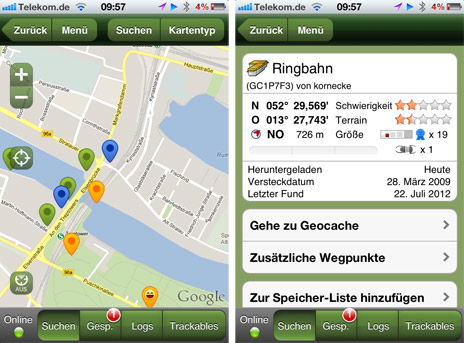
\includegraphics[width=0.65\textwidth]{2-Spielideen/2-3-Related_Work/geocaching-app.png}
   %  \caption{Die Geocaching-App. Auf der Karte werden verschiedene Caches dargestellt. Rechts sieht man Details zu einem ausgew�hlten Cache.
	%	(Quelle: \url{http://www.iphone-ticker.de/wp-content/uploads/2012/08/geocaching-app.jpg})
	%	}
%\end{figure}